\documentclass[tikz,border=2pt]{standalone}
\usepackage{amsmath,amssymb}
\usepackage{mathptmx}
\usetikzlibrary{arrows.meta,calc}
\definecolor{lab}{HTML}{0072B2}\definecolor{raw}{HTML}{E69F00}\definecolor{sil}{HTML}{777777}
\definecolor{water}{HTML}{56B4E9}\definecolor{dry}{HTML}{D9C79A}\definecolor{verm}{HTML}{D55E00}
% small labels at 6 pt so they stay legible at column width
\renewcommand{\tiny}{\fontsize{6}{7}\selectfont}
\begin{document}
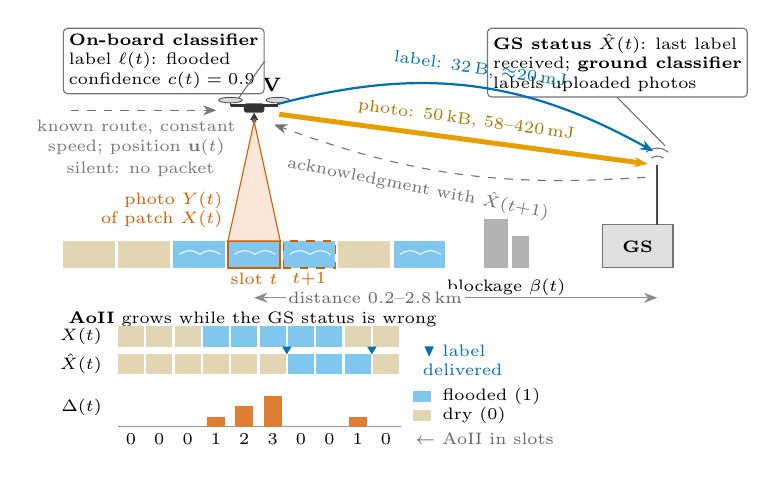
\begin{tikzpicture}[font=\scriptsize, >={Stealth[length=1.7mm]}]
% ---------------- ground patches ----------------
\def\pw{0.7}
\foreach \i in {0,1,5}{\fill[dry!75] (\i*\pw,0) rectangle ++(\pw-0.04,0.34);}
\foreach \i in {2,3,4,6}{\fill[water!75] (\i*\pw,0) rectangle ++(\pw-0.04,0.34);
  \draw[white,line width=0.35pt] (\i*\pw+0.08,0.17) sin ++(0.13,0.05) cos ++(0.13,-0.05) sin ++(0.13,0.05) cos ++(0.13,-0.05);}
\draw[verm, line width=0.8pt] (3*\pw,0) rectangle ++(\pw-0.04,0.34);
\draw[verm, dashed, line width=0.5pt] (4*\pw,0) rectangle ++(\pw-0.04,0.34);
\node[font=\tiny, text=verm] at (3*\pw+0.33,-0.14) {slot $t$};
\node[font=\tiny, text=verm] at (4*\pw+0.33,-0.14) {$t{+}1$};
% ---------------- UAV ----------------
\coordinate (uav) at (2.43,2.0);
\begin{scope}[shift={(uav)}]
  \draw[black!80, line width=0.9pt] (-0.30,0.06) -- (0.30,0.06);
  \foreach \x in {-0.30,0.30}{\draw[black!80] (\x,0.06) -- (\x,0.12);
     \fill[black!15] (\x,0.13) ellipse (0.15 and 0.035); \draw[black!70, line width=0.3pt] (\x,0.13) ellipse (0.15 and 0.035);}
  \fill[black!80, rounded corners=1pt] (-0.13,-0.03) rectangle (0.13,0.09);
  \fill[black!80] (0,-0.03) -- (-0.05,-0.12) -- (0.05,-0.12) -- cycle;
  \fill[black!60] (0,-0.13) circle (0.03);
\end{scope}
\node[font=\scriptsize\bfseries] at ($(uav)+(0,0.33)$) {UAV};
\draw[->, sil, dashed] (0.1,2.0) -- (1.95,2.0) node[pos=0.45, below, font=\tiny, text=sil, align=center] {known route, constant\\speed; position $\mathbf{u}(t)$};
% footprint
\fill[verm!15] ($(uav)+(0,-0.14)$) -- (3*\pw,0.35) -- (4*\pw-0.04,0.35) -- cycle;
\draw[verm, thin] ($(uav)+(0,-0.14)$) -- (3*\pw,0.35) ($(uav)+(0,-0.14)$) -- (4*\pw-0.04,0.35);
\node[font=\tiny, text=verm, align=right, anchor=east] at (2.15,0.74) {photo $Y(t)$\\of patch $X(t)$};
% on-board classifier callout
\node[draw=black!55, fill=white, rounded corners=1.5pt, align=left, inner sep=2pt, font=\tiny, anchor=north west] (cls) at (0.0,3.05)
  {\textbf{On-board classifier}\\label $\ell(t)$: flooded\\confidence $c(t)=0.9$};
\draw[black!55] (cls.east) -- ($(uav)+(-0.2,0.15)$);
\node[font=\tiny, text=sil, anchor=east] at (2.05,1.25) {silent: no packet};
% ---------------- obstacle ----------------
\fill[black!30] (5.35,0) rectangle ++(0.3,0.62); \fill[black!30] (5.7,0) rectangle ++(0.22,0.4);
\node[font=\tiny, anchor=north] at (5.63,-0.02) {blockage $\beta(t)$};
% ---------------- GS ----------------
\coordinate (ant) at (7.55,1.3);
\fill[black!12] (6.85,0) rectangle (7.75,0.55); \draw[black!55] (6.85,0) rectangle (7.75,0.55);
\node[font=\tiny\bfseries] at (7.3,0.27) {GS};
\draw[black!70, line width=0.7pt] (7.55,0.55) -- (ant);
\foreach \r in {0.12,0.22}{\draw[black!55] (ant) ++(50:\r) arc (50:130:\r);}
\node[draw=black!55, fill=white, rounded corners=1.5pt, align=left, inner sep=2pt, font=\tiny, anchor=north east] (gs) at (8.7,3.05)
  {\textbf{GS status} $\hat X(t)$: last label\\received; \textbf{ground classifier}\\labels uploaded photos};
\draw[black!55] (gs.south) -- ($(ant)+(0.1,0.25)$);
% ---------------- actions ----------------
\draw[->, lab, line width=0.8pt] ($(uav)+(0.3,0.08)$) to[bend left=22] node[pos=0.52, above, sloped, font=\tiny, text=lab] {label: 32\,B, ${\approx}20$\,mJ} ($(ant)+(-0.05,0.18)$);
\draw[->, raw, line width=1.8pt] ($(uav)+(0.32,-0.05)$) -- node[pos=0.5, above, sloped, font=\tiny, text=raw!75!black] {photo: 50\,kB, 58--420\,mJ} ($(ant)+(-0.12,0.02)$);
\draw[->, dashed, black!55] ($(ant)+(-0.15,-0.15)$) to[bend left=12] node[pos=0.6, below, sloped, font=\tiny] {acknowledgment with $\hat X(t{+}1)$} ($(uav)+(0.25,-0.18)$);
% distance
\draw[<->, black!45] (2.43,-0.38) -- node[pos=0.3, fill=white, inner sep=1pt, font=\tiny, text=black!60] {distance $0.2$--$2.8$\,km} (7.55,-0.38);
% ---------------- AoII inset ----------------
\begin{scope}[shift={(0,-2.12)}]
  \def\cw{0.36}
  \node[font=\tiny, anchor=west] at (-0.05,1.47) {\textbf{AoII} grows while the GS status is wrong};
  \node[font=\tiny, anchor=east] at (0.62,1.25) {$X(t)$};
  \node[font=\tiny, anchor=east] at (0.62,0.9) {$\hat X(t)$};
  \node[font=\tiny, anchor=east] at (0.62,0.35) {$\Delta(t)$};
  \foreach \x [count=\k from 0] in {0,0,0,1,1,1,1,1,0,0}{
     \ifnum\x=1 \fill[water!75] (0.7+\k*\cw,1.12) rectangle ++(\cw-0.03,0.26); \else \fill[dry!75] (0.7+\k*\cw,1.12) rectangle ++(\cw-0.03,0.26); \fi}
  \foreach \x [count=\k from 0] in {0,0,0,0,0,0,1,1,1,0}{
     \ifnum\x=1 \fill[water!75] (0.7+\k*\cw,0.77) rectangle ++(\cw-0.03,0.26); \else \fill[dry!75] (0.7+\k*\cw,0.77) rectangle ++(\cw-0.03,0.26); \fi}
  % delivered labels (between slots)
  \fill[lab] (0.7+6*\cw-0.015,1.05) ++(-0.06,0.07) -- ++(0.12,0) -- ++(-0.06,-0.1) -- cycle;
  \fill[lab] (0.7+9*\cw-0.015,1.05) ++(-0.06,0.07) -- ++(0.12,0) -- ++(-0.06,-0.1) -- cycle;
  % AoII bars
  \draw[black!40] (0.7,0.1) -- (0.7+10*\cw,0.1);
  \foreach \d [count=\k from 0] in {0,0,0,1,2,3,0,0,1,0}{
     \ifnum\d>0 \fill[verm!80] (0.7+\k*\cw+0.05,0.1) rectangle ++(\cw-0.13,0.13*\d); \fi
     \node[font=\tiny] at (0.7+\k*\cw+\cw/2-0.015,-0.05) {\d};}
  \node[font=\tiny, anchor=west, text=lab, align=left] at (0.85+10*\cw,0.95) {$\blacktriangledown$ label\\delivered};
  \fill[water!75] (0.85+10*\cw,0.42) rectangle ++(0.22,0.14); \node[font=\tiny, anchor=west] at (1.1+10*\cw,0.49) {flooded ($1$)};
  \fill[dry!75] (0.85+10*\cw,0.18) rectangle ++(0.22,0.14); \node[font=\tiny, anchor=west] at (1.1+10*\cw,0.25) {dry ($0$)};
  \node[font=\tiny, anchor=west, text=black!60] at (0.75+10*\cw,-0.05) {$\leftarrow$ AoII in slots};
\end{scope}
\end{tikzpicture}
\end{document}
